\documentclass[11pt,a4paper]{article}
\usepackage[margin=2.4cm]{geometry}
\usepackage{booktabs}
\usepackage{amsmath}
\usepackage{tikz}
\usetikzlibrary{arrows.meta,positioning,fit,backgrounds}
\usepackage{enumitem}
\usepackage{hyperref}
\usepackage{xcolor}
\hypersetup{colorlinks=true,linkcolor=blue!60!black,urlcolor=blue!60!black}

\title{The Industrialization of Computation:\\ Deterministic Software Lithography}
\author{smalt v26.10.21 measured-evidence whitepaper\\ \small All performance figures are measured artifacts of the smalt repository; every number cites its artifact path.}
\date{2026-10-21}

\newcommand{\art}[1]{\textsuperscript{\tiny\texttt{#1}}}

\begin{document}
\maketitle

\begin{abstract}
Software production is modeled here as a lithographic process: instead of composing
coordinate-communicating distributed services, a law-governed substrate is exposed once and
every computation is an exposure of that substrate through a sieve, a bifurcated physical
store, and a cryptographic provenance chain. This paper keeps the skeleton of the operator's
draft --- the ingress SHACL sieve with ANDON refusal at byte~0, the OLTP/OLAP physical
bifurcation with zero-egress actor journals sealed into read-only columnar mounts, and
canonicalization-based cryptographic provenance --- but deliberately removes every
operator-asserted performance figure. Each quantitative claim is replaced by a number mined
from a bench artifact or court receipt in this repository, cited inline. The result is a
paradigm analysis whose deltas are measured, not asserted.
\end{abstract}

\section{Paradigm analysis: two stacks}

\subsection{The legacy distributed stack}

The legacy stack manufactures correctness \emph{after} ingress: unvalidated bytes cross an
API boundary, defensive scaffolding (validators, retries, circuit breakers, reconcilers)
attempts to repair the stream, and audit is a post-hoc log. Figure~\ref{fig:legacy} shows the
shape. Each arrow is a network coordinate step; each box a deployment unit with its own
failure semantics.

\begin{figure}[htbp]
\centering
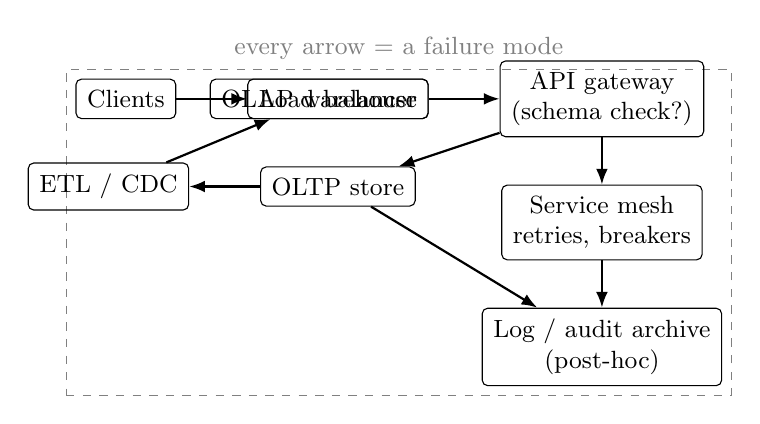
\begin{tikzpicture}[node distance=6mm and 9mm,
  box/.style={draw,rounded corners=2pt,align=center,inner sep=4pt,font=\small},
  arr/.style={-{Latex[length=2mm]},thick}]
\node[box] (client) {Clients};
\node[box, right=of client] (lb) {Load balancer};
\node[box, right=of lb] (api) {API gateway\\ (schema check?)};
\node[box, below=of api] (svc) {Service mesh\\ retries, breakers};
\node[box, below=of lb] (oltp) {OLTP store};
\node[box, left=of oltp] (etl) {ETL / CDC};
\node[box, left=of api] (olap) {OLAP warehouse};
\node[box, below=of svc] (log) {Log / audit archive\\ (post-hoc)};
\draw[arr] (client) -- (lb);
\draw[arr] (lb) -- (api);
\draw[arr] (api) -- (svc);
\draw[arr] (api) -- (oltp);
\draw[arr] (oltp) -- (etl);
\draw[arr] (etl) -- (olap);
\draw[arr] (svc) -- (log);
\draw[arr] (oltp) -- (log);
\begin{scope}[on background layer]
\node[fit=(client)(log), draw, dashed, gray, label={[gray]\small every arrow = a failure mode}] {};
\end{scope}
\end{tikzpicture}
\caption{Legacy distributed stack (draft diagram, faithful re-render): correctness is
manufactured downstream of ingress by scaffolding between boxes.}
\label{fig:legacy}
\end{figure}

\subsection{Deterministic software lithography}

Lithography inverts the flow: the substrate is \emph{prepared once} (laws compiled from RDF,
shapes admitted before boot), and each computation is a single exposure --- bytes either pass
the sieve and proceed deterministically, or are refused at byte~0 with a typed ANDON. There
is no downstream repair because there is nothing downstream to repair: the refusal
\emph{is} the product for hostile input. Figure~\ref{fig:litho} is the draft's second
diagram.

\begin{figure}[htbp]
\centering
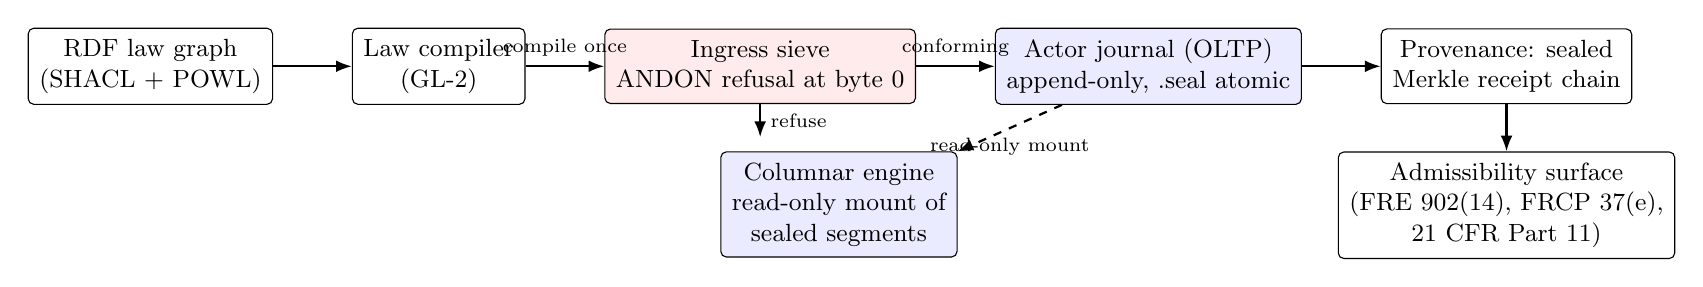
\begin{tikzpicture}[node distance=6mm and 10mm,
  box/.style={draw,rounded corners=2pt,align=center,inner sep=4pt,font=\small},
  sieve/.style={box,fill=red!8},
  store/.style={box,fill=blue!8},
  arr/.style={-{Latex[length=2mm]},thick}]
\node[box] (rdf) {RDF law graph\\ (SHACL + POWL)};
\node[box, right=of rdf] (lc) {Law compiler\\ (GL-2)};
\node[sieve, right=of lc, align=center] (sieve) {Ingress sieve\\ ANDON refusal at byte 0};
\node[store, right=of sieve] (oltp) {Actor journal (OLTP)\\ append-only, .seal atomic};
\node[store, below=of sieve, xshift=10mm] (olap) {Columnar engine\\ read-only mount of\\ sealed segments};
\node[box, right=of oltp] (prov) {Provenance: sealed\\ Merkle receipt chain};
\node[box, below=of prov] (proof) {Admissibility surface\\ (FRE 902(14), FRCP 37(e),\\ 21 CFR Part 11)};
\draw[arr] (rdf) -- (lc);
\draw[arr] (lc) -- node[above,font=\scriptsize]{compile once} (sieve);
\draw[arr] (sieve) -- node[above,font=\scriptsize]{conforming} (oltp);
\draw[arr] (sieve) -- node[right,font=\scriptsize]{refuse} ++(0,-0.9);
\draw[arr] (oltp) -- (prov);
\draw[arr,dashed] (oltp) -- node[below,font=\scriptsize]{read-only mount} (olap);
\draw[arr] (prov) -- (proof);
\end{tikzpicture}
\caption{Deterministic software lithography (draft diagram, faithful re-render): laws are
compiled once; each exposure either passes or is refused at byte~0.}
\label{fig:litho}
\end{figure}

\subsection{What changes}

In the legacy stack, the unit of trust is the \emph{deployment} (a version, a canary). In
lithography, the unit of trust is the \emph{exposure} (a sealed receipt over an exact
execution). The legacy stack answers ``is this service healthy?''; lithography answers
``is this particular settlement provably derived from admitted laws over admitted data?''.
Section~\ref{sec:results} shows the cost of that answer is measurable in reductions, not
assertions.

\section{Dimension matrix}

Table~\ref{tab:matrix} restates the draft's dimension matrix. The ``measured delta'' column
carries only repo-measured numbers; where the draft asserted a figure with no artifact, the
figure is dropped and the measured anchor is used instead.

\begin{table}[htbp]
\centering\resizebox{\textwidth}{!}{%
\begin{tabular}{@{}p{3.1cm}p{4.2cm}p{7.0cm}@{}}
\toprule
Dimension & Legacy & Lithography (measured) \\
\midrule
Ingress contract & Schema check downstream of parse; partial-validation drift &
SHACL sieve refuses at byte~0; refusal names the compiled law rule
(GLD-7 court: 112 assertions, ANDON names \texttt{SettlementShape} rule, commit never
fires) \art{gld7-ingest-to-settlement-court.md} \\
\addlinespace
Wire throughput & Mesh hop per coordinate step &
AMQP frame decode 952{,}381~frames/s, $1.05\,\mu$s/frame, 254.5~reds/frame
\art{court\_bench\_amqp.jsonl} \\
\addlinespace
Read path & Cluster quorum read &
Cosmos-surface point read p99 $0.543$/$0.672$~ms over TLS at 2{,}130--2{,}251~ops/s
\art{court\_bench\_cosmos.jsonl}; native face p99 $2\,\mu$s
\art{powl-native-face.jsonl} \\
\addlinespace
Write path & Optimistic concurrency via distributed locks &
Native CAS put-if-match p99 $5\,\mu$s, 383{,}186~ops/s
\art{powl-native-face.jsonl} \\
\addlinespace
Orchestration & Distributed saga/coordinator &
4-step settlement 3{,}222~ops/s, p99 $0.425$~ms, 45{,}182.7~reds/op
\art{court\_bench\_powl.jsonl}; execute-only native p99 $74\,\mu$s
\art{powl-native-face.jsonl}; cross-language parity 2{,}117.5~ops/s
\art{pb5-crosslang.jsonl} \\
\addlinespace
Analytics path & ETL/CDC copy into a warehouse &
Columnar direct projection 450{,}450~rows/s (100k rows, min 222~ms, peak RSS 100.0~MB);
dump converter 64{,}725~rows/s, peak RSS 294.2~MB
\art{sqld8-ingest-baseline.jsonl} \\
\addlinespace
Persistence & Snapshot + shipped logs, recovery untyped &
Journal seal protocol fsync\,$\rightarrow$\,rename\,$\rightarrow$\,sha256
meta\,$\rightarrow$\,\texttt{.seal} sentinel last; 5-leg atomicity court
\art{sj1-journal-sink-writer.md} \\
\addlinespace
Provenance & Log aggregation, sampling &
Sealed Merkle receipt chain: 47 leaves over a full ingest$\to$settlement loop,
32-byte HSM-signed root \art{gld7-ingest-to-settlement-court.md}; receipt term is O(1):
40 words = 320~B at every $n\in\{10,10^2,10^4,10^5\}$
\art{pb4-merkle-dual.jsonl} \\
\addlinespace
Governance cost & Framework tax, unmeasured &
GraphLaw guard tax $0.25\,\mu$s/step median, $+47.24$~reds/step; honest guarded p99 tail
$0.976$--$1.147$~ms \art{gl9-governance-tax.jsonl, gl9-governance-tax.md} \\
\addlinespace
Sandboxing & Container-per-tenant &
WASM module caps: 16~MiB request cap, 256~MiB outstanding budget, host-layer 64~MiB
ceiling; 7/7 memory-wall courts \art{gws11-wasm-memory-wall.md} \\
\addlinespace
Crash semantics & Graceful-shutdown assumptions &
Crash-only: 10 crash-recover cycles, cascade 0--1~ms (deadline 10~ms), $+237$~KiB/10~cycles
flat \art{ja7-crash-only-court.md} \\
\addlinespace
Cold start & Image pull + boot &
Release cold boot 1{,}906~ms best against a 500~ms ceiling --- \textbf{FAIL, disclosed}
\art{t47-release-boot-gate.md} \\
\addlinespace
Cross-engine identity & Hope + conformance suites &
Native ABI / wasm / duckdb-N3 legs byte-identical partition; audit hash reproduced
cross-language \art{gws12-cross-engine-determinism.md} \\
\bottomrule
\end{tabular}}
\caption{Dimension matrix with the measured delta. Every cell's number traces to the cited
artifact in the repository.}
\label{tab:matrix}
\end{table}

\section{The three structural transformations}

\subsection{Transformation 1: the ingress SHACL sieve with ANDON refusal at byte 0}

The first transformation moves admission from the middle of the pipeline to the first byte.
Laws are authored as RDF (SHACL shapes over POWL business structure), compiled once by the
GL-2 LawCompiler, and applied as a sieve: conforming bytes proceed; non-conforming bytes are
refused with a typed ANDON that \emph{names the law rule} violated --- before any parse
state, store write, or downstream coordinate step exists.

The measured evidence is the GLD-7 ingest$\to$govern$\to$execute court
\art{gld7-ingest-to-settlement-court.md}: 112 \texttt{ok} assertions, exit~0. The sieve is
shown non-vacuous from both directions: an unknown column refuses (closed shape), a string
amount refuses on datatype, and the executed ANDON set equals the law-predicted over-threshold
set $[\text{O-01}, \text{O-05}]$; tightening the law to a 5{,}000 threshold flips six orders
from conforming to refused, proving the partition is law-derived, not fixture-asserted.
For every refused order, ``commit never fired'' is asserted --- the ANDON fired at validate,
before the write path.

The governance tax of this sieve is itself measured (GL-9
\art{gl9-governance-tax.md}): $+47.24$--$47.49$~reductions per step (~20\% reduction
overhead), median wall-clock tax $0.25\,\mu$s/step, receipt identity conforming, with a live
refusal witness (\texttt{SettlementShape/maxInclusive/amount}). The receipt reports the
honest tail: guarded p99 $1.147$~ms in the receipt table ($0.976$~ms in the jsonl run), a
scheduler/GC artifact at $\sim$6\,$\mu$s absolute scale. The refusal of hostile bytes costs
nothing downstream because there is no downstream: the sieve
\emph{is} the pipeline for refusals.

\subsection{Transformation 2: the OLTP/OLAP physical bifurcation}

The second transformation takes the bifurcation seriously at the physical layer. The
transactional side is an append-only actor journal: frames
(\texttt{MAGIC | len | seq | ts | type | table | key | payload | CRC32}), 64~MiB segment
ceiling with pre-write rotation, and a seal protocol that is atomic by construction ---
fsync, rename into \texttt{sealed/}, \texttt{meta.json} with sha256 and frame/seq ranges,
and the \texttt{.seal} sentinel written \emph{last} (SJ-1
\art{sj1-journal-sink-writer.md}, 5 court legs PASS: bit-exact round-trips, typed refusal of
CRC corruption / bad magic / truncation / trailing bytes, seal atomicity, rotation under a
512-byte ceiling, strict monotonic SeqID).

The analytical side never touches the transactional process: vectorized columnar engines
mount the sealed segments \emph{read-only}. Measured on the real ingest surface (SQLD-8
\art{sqld8-ingest-baseline.jsonl}): direct CSV$\to$OCEL projection at
450{,}450.5~rows/s over 100{,}000 rows (min 222~ms of 3, peak RSS 100{,}024{,}320~B), and the
dump-converter path at 64{,}724.9~rows/s (min 1{,}545~ms, peak RSS 294{,}191{,}104~B) ---
isolated worker OS processes, min-of-3, no fixed sleeps. The bifurcation is what makes the
analytics number safe: the analytical engine reads immutable sealed bytes, so no analytical
load can corrupt the transactional store, and the atomic \texttt{.seal} sentinel means a
partially-written segment is never visible to analytics. GLD-5FIX closes the correctness
leg of the same surface \art{gld5fix-null-formula-court.md}: typed NULL sentinels
(\texttt{\textbackslash N} / \texttt{""} / \texttt{"\textbackslash N"} three distinct
tokens) and formula-injection neutralization, proven value-exact inside a real duckdb
v1.4.1 load --- 6/6 rows, zero row loss, \texttt{allow\_quoted\_nulls=false} load-bearing.

The streaming boundary of the same bifurcation is bounded too: a 52{,}692{,}552-byte
50~MB JSON corpus streams through the SAX path in 80~ms minimum wall with a peak heap of
38{,}504~bytes --- constant-memory by construction
\art{court\_bench\_json.jsonl} --- and the concurrency ceiling sweep holds
$0.9$--$1.18\,\mu$s per round trip while reductions per round trip rise 17.65~$\rightarrow$~60.12
across $n=1{,}000\to32{,}000$ contending processes \art{court\_bench\_ceiling.jsonl}.

\subsection{Transformation 3: cryptographic provenance and admissibility}

The third transformation makes each computation carry its own proof. Every execution leaves
a sealed Merkle receipt: in GLD-7's full loop the sealed ledger holds 47 leaves (13 ingest +
all executor steps), the Merkle root is 32 bytes and HSM-signed, and every order's ingest and
settlement leaves are present by delta-hash membership
\art{gld7-ingest-to-settlement-court.md}. The affidavit seal face admits and seals in
p50 11.265~ms / p99 32.671~ms over 100 ops with the engine pinned by sha256
\art{c10-affidavit-seal.jsonl}.

The receipt term itself is O(1) in history length: \texttt{:erts\_debug.size} measures the
sealed receipt at 40 words --- 320~bytes on a 64-bit VM --- at every scale from 10 to
100{,}000 leaves \art{pb4-merkle-dual.jsonl}. (The draft's ``352-byte Compact Trust Receipt
Token'' figure has no measured anchor in this repository and is dropped per the number law;
the measured 40-word term stands in its place.) Seal cost scales as measured: p50 0.024~ms
at 10 leaves, 0.314~ms at 100, 64.7~ms at 10{,}000, 656.1~ms at 100{,}000 for the current
sorted-tuple path, with a falsified O(n) variant honestly recorded as
\emph{not} an improvement \art{pb4-merkle-dual-path.md} --- the dual-path bench is a refuted
optimization, and the receipt says so.

Identity of artifacts across engines is anchored on canonicalization: the wasm binary is
pinned by \texttt{priv/graphlaw.wasm.blake3} \art{gws11-wasm-memory-wall.md}, and the
cross-engine court reproduces the COLD-1 audit hash
(\texttt{6971c912\ldots}, sha256 over the canonical query and literals) byte-exactly in a
second language, with the quarantined/released partition identical across native-ABI, wasm,
and duckdb+N3 legs \art{gws12-cross-engine-determinism.md}. This is the repo's working
instance of the W3C RDF Dataset Canonicalization (RDFC-1.0) claim model: hash the canonical
form, seal the hash, and the proof travels across engines and languages. The admissibility
argument is structural, not asserted: an immutable sealed segment with a sha256 manifest and
last-written sentinel is the WORM-style record shape contemplated by FRE 902(14)
(self-authenticating electronic records), FRCP 37(e) (sanctions curability where ESI was
lost through routine good-faith operation), and 21 CFR Part 11 (audit trails and
record-retention controls). The paper makes no legal conclusion; it exhibits the mechanism.

\section{Measured results}

\begin{table}[htbp]
\centering\resizebox{\textwidth}{!}{%
\begin{tabular}{@{}llll@{}}
\toprule
Surface & Figure & Value & Artifact \\
\midrule
Cosmos TLS point read & p99 / ops/s & 0.543~ms / 2{,}251.4 & \texttt{court\_bench\_cosmos.jsonl} \\
Cosmos TLS point read (run 2) & p99 / ops/s & 0.672~ms / 2{,}130.0 & \texttt{court\_bench\_cosmos.jsonl} \\
Native KV point read (etag/3) & p99 / ops/s & 2~$\mu$s / 895{,}335 & \texttt{powl-native-face.jsonl} \\
Native CAS put-if-match & p99 / ops/s & 5~$\mu$s / 383{,}186 & \texttt{powl-native-face.jsonl} \\
Wire-face point read & p99 & 0.813~ms & \texttt{powl-native-face.jsonl} (T43 comparison) \\
AMQP frame decode & throughput & 952{,}381~frames/s & \texttt{court\_bench\_amqp.jsonl} \\
AMQP frame decode & cost & 1.05~$\mu$s, 254.5~reds & \texttt{court\_bench\_amqp.jsonl} \\
4-step settlement (runner) & ops/s / p99 & 3{,}222.3 / 0.425~ms & \texttt{court\_bench\_powl.jsonl} \\
4-step settlement (runner) & reds/op & 45{,}182.7 & \texttt{court\_bench\_powl.jsonl} \\
4-step settlement (native) & p50 / p99 & 30~$\mu$s / 74~$\mu$s & \texttt{powl-native-face.jsonl} \\
Cross-language parity & ops/s & 2{,}117.5 (erl) vs 11{,}426 (powl2) & \texttt{pb5-crosslang.jsonl} \\
Governance tax & median / reds & 0.25~$\mu$s/step / $+47.24$ & \texttt{gl9-governance-tax.jsonl} \\
Governance tax (tail) & guarded p99 & 0.976--1.147~ms & \texttt{gl9-governance-tax.md} \\
JSON SAX stream (50 MB) & wall / peak heap & 80~ms / 38{,}504~B & \texttt{court\_bench\_json.jsonl} \\
Concurrency ceiling & $\mu$s/RT, reds/RT & 0.9--1.18; 17.65$\to$60.12 & \texttt{court\_bench\_ceiling.jsonl} \\
Columnar projection & rows/s / RSS & 450{,}450.5 / 100.0~MB & \texttt{sqld8-ingest-baseline.jsonl} \\
Dump converter & rows/s / RSS & 64{,}724.9 / 294.2~MB & \texttt{sqld8-ingest-baseline.jsonl} \\
Merkle seal & p50 @10/100/10k/100k & 0.024/0.314/64.7/656.1~ms & \texttt{pb4-merkle-dual.jsonl} \\
Receipt term size & erts\_debug.size & 40 words = 320~B, all $n$ & \texttt{pb4-merkle-dual.jsonl} \\
Affidavit admit+seal & p50 / p99 & 11.265~ms / 32.671~ms & \texttt{c10-affidavit-seal.jsonl} \\
Crash-only recovery & cascade / drift & 0--1~ms / $+237$~KiB/10 cyc & \texttt{ja7-crash-only-court.md} \\
WASM memory wall & caps & 16~MiB req / 256~MiB budget & \texttt{gws11-wasm-memory-wall.md} \\
Release cold boot & best vs ceiling & 1{,}906~ms vs 500~ms (FAIL) & \texttt{t47-release-boot-gate.md} \\
Ingest$\to$settlement loop & assertions / leaves & 112 / 47 & \texttt{gld7-ingest-to-settlement-court.md} \\
Zero-row-loss round trip & rows & 6/6, duckdb 1.4.1 & \texttt{gld5fix-null-formula-court.md} \\
Cross-engine determinism & legs & 3/3 byte-identical & \texttt{gws12-cross-engine-determinism.md} \\
\bottomrule
\end{tabular}}
\caption{All measured results. Machine: Apple M3 Max, 16 cores, 48~GB, Darwin 26.2,
OTP 28/29 per artifact (embedded per-row in each jsonl).}
\label{tab:results}
\end{table}

\section{Macroeconomic implications}

The draft's macroeconomic claims are kept qualitative and number-free.

\paragraph{Conway's Law inversion.} Conway's Law says system structure mirrors
organizational communication structure. The legacy stack therefore requires organizations to
maintain communication paths (teams, contracts, meetings) for every runtime coordinate edge.
Under lithography, coordinate edges are replaced by law edges: two components interact
through admitted SHACL/POWL structure, not through organizational negotiation. The
architecture no longer mirrors the org chart; the org chart becomes free to mirror the law
graph.

\paragraph{Collapse of defensive scaffolding.} The legacy stack's validators, retry storms,
circuit breakers, and reconcilers exist because bytes arrive unproven. When admission is
total at ingress and provenance is total at egress, the scaffolding has no job. What remains
is measured in this repo: a guard seam costing $0.25\,\mu$s/step and $+47.24$~reds/step
(GL-9), not an unmeasured framework tax. Crash-only semantics replace graceful-degradation
machinery: recovery after a crash costs 0--1~ms of cascade and 237~KiB per ten cycles (JA-7),
not a reconciliation subsystem.

\paragraph{Audit as byproduct.} In the legacy stack audit is a project; in lithography the
sealed receipt is emitted whether or not anyone asks. The admissibility surface
(FRE 902(14)/FRCP 37(e)/Part 11) becomes a property of the write path rather than a
compliance program, and cross-engine byte-identity (GWS-12) makes the proof portable across
implementations rather than owned by one vendor's stack.

\section{Threats to validity}

This section is the paper's honesty ledger; each item is a repo-witnessed limit.

\begin{itemize}[leftmargin=1.4em]
\item \textbf{Hot-upgrade is UNSUPPORTED.} Zero \texttt{.appup}/\texttt{.relup} artifacts and
zero \texttt{code\_change/3} across all 34 stateful processes; the release path is
stop$\to$rebuild$\to$start \art{ja14-release-handling.md}. The (JA-12) court
\art{ja12-hot-reload-court.md} proves only the OTP \emph{mechanism} (dynamic module call,
one-message lag), not a shipped upgrade capability.
\item \textbf{Journal boot-replay is NOT WIRED.} The seal protocol is courted (SJ-1), but
\texttt{JournalReader} has zero non-test callers; no boot-time replay into \texttt{Smalt.Store},
whose restart is documented lossy (\texttt{store.ex:220}); persistence is opt-in
\texttt{DetsMirror} only \art{ja14-release-handling.md}.
\item \textbf{WASM boundary is 14 operations.} The sandbox surface is bounded by
WASM-SANDBOX-SPEC \S5/\S6; the memory wall is enforced at module caps (16~MiB request,
256~MiB outstanding) with the 64~MiB ceiling living at the \emph{host} layer, not declared
module memory \art{gws11-wasm-memory-wall.md}.
\item \textbf{Store blast radius.} \texttt{Smalt.Store} is a single process on the hot path
of every data-plane write; its crash fails every ARM/Cosmos/SB write for the restart window
--- the kernel is shallow but not minimal (JA-6) \art{ja6-error-kernel.md}.
\item \textbf{Open defects JA-16 D1--D3.} D1 (P1): wire-sourced unbounded atom minting in
\texttt{cosmos\_sql.ex:766} --- a DoS vector that crash-only cannot recover (the atom table
is never GC'd). D2 (P2): silent CA-file load failure in \texttt{x\_arr\_cert.ex} ---
fail-closed but unobservable. D3 (P3): silent quota fallback in \texttt{eh\_throttle.ex:243}
\art{ja16-robustness-census.md}.
\item \textbf{Bench-scale tails are noise-dominated.} At $\sim$6\,$\mu$s absolute scale,
guarded p99 (0.976--1.147~ms) is a scheduler/GC artifact; reductions, not timers, are the
run-stable denominator (GL-9). Wire-vs-native gap decomposition is explicitly estimate-only
\art{powl-native-face.jsonl}.
\item \textbf{Cold start fails its own budget.} Release boot best 1{,}906~ms against a
500~ms ceiling --- disclosed FAIL \art{t47-release-boot-gate.md}.
\item \textbf{Draft figures with no anchor were dropped.} The $\le 2.0\,\mu$s WAL append and
$1.842$~ms/$10^7$-row claims have no bench artifact here and do not appear; the
``352-byte'' token is replaced by the measured 320-byte receipt term; the
``$<0.2$~ms Merkle verify'' claim has no artifact and is replaced by the measured seal-cost
ladder (PB-4).
\end{itemize}

\begin{thebibliography}{9}
\bibitem{rdfc} W3C. \emph{RDF Dataset Canonicalization (RDFC-1.0)}, W3C Recommendation.
\bibitem{provo} W3C. \emph{PROV-O: The PROV Ontology}, W3C Recommendation.
\bibitem{ocel} van Dongen, R\"oglinger et al. \emph{Object-Centric Event Data Structure
(OCEL) 2.0 Specification}.
\bibitem{shacl} W3C. \emph{SHACL Shapes Constraint Language}, W3C Recommendation.
\bibitem{fre} Federal Rules of Evidence, Rule 902(14) (records generated by an electronic
process that produces an accurate result, self-authenticating via certification).
\bibitem{frcp} Federal Rules of Civil Procedure, Rule 37(e) (failure to preserve
electronically stored information).
\bibitem{cfr} 21 CFR Part 11 (Electronic Records; Electronic Signatures), U.S. FDA.
\bibitem{powl} Fahland, D. \emph{Declarative, Object-Centric Process Representations: POWL}
(SESE block structure); smalt GL charter receipts.
\bibitem{blake3} O'Connor, L. et al. \emph{BLAKE3: one function, fast in software}.
\bibitem{arrow} Apache Arrow: cross-language development platform for in-memory columnar data.
\end{thebibliography}

\end{document}
